
%(BEGIN_QUESTION)
% Copyright 2006, Tony R. Kuphaldt, released under the Creative Commons Attribution License (v 1.0)
% This means you may do almost anything with this work of mine, so long as you give me proper credit

Fullfør følgende ladderlogiske skjemategning for en del av et nivåreguleringssystem for et kjølevannsreservoar, ved å sette inn riktige typer nivåbrytere på riktige steder, inkludert alle nødvendige forbindelsesledninger:

$$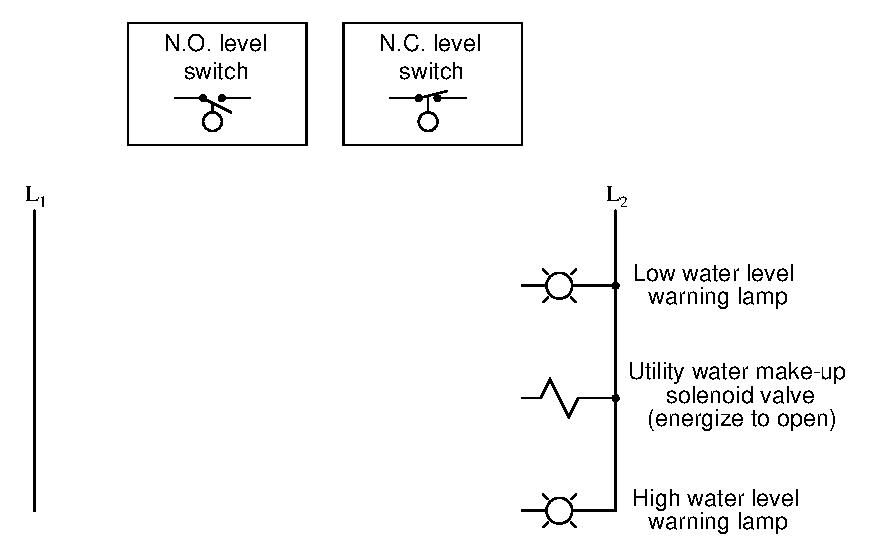
\includegraphics[width=15.5cm]{i00515x01.eps}$$

En nivåbryter, satt til 3 fot, styrer varselampe for lav vannstand og tenner lampen dersom vannnivået synker under 3 fot i reservoaret. En annen nivåbryter, satt til 2 fot, styrer påfyllingsventilen for forsyningsvann og åpner ventilen for å fylle på mer rent vann dersom nivået synker under 2 fot. Den siste nivåbryteren er satt til 5 fot og styrer varselampe for høy vannstand ved å tenne lampen dersom nivået stiger over 5 fot i reservoaret.

\vskip 10pt

\noindent
Poeng gis for korrekt kobling av hver av de tre grein-kretsene. Du {\it må} skrive oppgitt nivåinnstilling (i fot) ved hver bryter for å få poeng for den aktuelle kretsen:

\begin{itemize}
\item{} Varsellampe for lav vannstand
\item{} Magnetventil for påfyllingsvann
\item{} Varsellampe for høy vannstand
\end{itemize}

\underbar{file i00515}
%(END_QUESTION)





%(BEGIN_ANSWER)

$$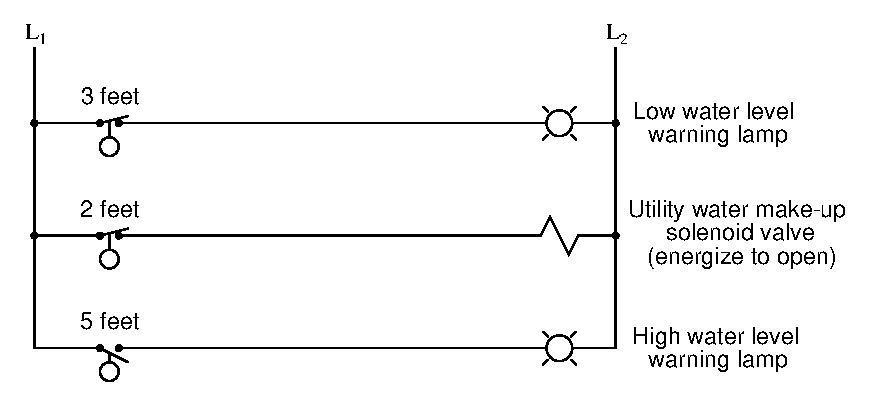
\includegraphics[width=15.5cm]{i00515x02.eps}$$

3 poeng for hver varselbryter, 4 poeng for magnetventilbryteren.

%(END_ANSWER)





%(BEGIN_NOTES)

{\bf Denne oppgaven er ment for eksamen, ikke arbeidsark!}.

%(END_NOTES)

